\documentclass[14pt, a4paper]{extarticle}
\usepackage{cmap}
\usepackage[14pt]{extsizes}
\usepackage[T2A]{fontenc}
%\usepackage[cp1251]{inputenc}
\usepackage{multirow}
\usepackage[utf8]{inputenc}
\usepackage[russian]{babel}
\usepackage{textcomp}
\usepackage {indentfirst} %красная строка
\setlength\parindent{1cm}
\usepackage{textcomp}
\usepackage{array}
\usepackage{amssymb}
\usepackage{amstext}
\usepackage{amsmath}
%\usepackage{ upgreek }
\usepackage{amsfonts}
\usepackage{amsthm}
\usepackage{euscript}
\usepackage{graphicx}
\usepackage{pscyr}
\pagestyle{myheadings}
\usepackage{geometry}
\geometry{left = 2.5cm}
\geometry{right = 2cm}
\geometry{top = 2cm}
\geometry{bottom = 2cm}
\geometry{mag=1000}
\geometry{headsep=0.7cm}
\geometry{footskip=1cm}

\renewcommand{\baselinestretch}{1.5}


\makeatletter
\@addtoreset{equation}{section} % Счетчик формул
\numberwithin{equation}{section}
\makeatother
\renewcommand{\rmdefault}{ftm}

\makeatletter
\renewcommand{\l@section}{\@dottedtocline{1}{0.6cm}{0.6cm}}
\renewcommand{\thesection}{\arabic{section}}
\renewcommand{\section}{\@startsection{section}{1}{1.25cm}{-3.5ex plus -1ex minus -.2ex}{2.3ex plus.2ex}{\center\normalfont}}
\makeatother

%Оформление подразделов
\makeatletter
\renewcommand{\l@subsection}{\@dottedtocline{2}{0.8cm}{0.8cm}}
\renewcommand{\thesubsection}{\arabic{section}.\arabic{subsection}}
\renewcommand{\subsection}{\@startsection{subsection}{2}{1.25cm}{-3.5ex plus -1ex minus -.2ex}{2.3ex plus.2ex}{\center\normalsize}}
\makeatother

%Оформление под-подразделов
\makeatletter
\renewcommand{\thesubsubsection}{\arabic{section}.\arabic{subsection}.\arabic{subsubsection}}
\renewcommand{\subsubsection}{\@startsection{subsubsection}{3}{1.25cm}{-3.5ex plus -1ex minus -.2ex}{2.3ex plus.2ex}{\center\normalsize}}
\makeatother


\DeclareMathOperator{\conv}{conv}
\DeclareMathOperator{\Lin}{Lin}
\DeclareMathOperator{\diam}{diam}
\DeclareMathOperator{\Aff}{Aff}
\DeclareMathOperator{\Ext}{Ext}
\DeclareMathOperator{\card}{card}
\DeclareMathOperator{\sign}{sign}
\DeclareMathOperator*{\argmin}{arg ~ min}
\DeclareMathOperator*{\argmax}{arg ~ max}
\renewcommand{\baselinestretch}{1.5}
\setcounter{page}{2}


\title{Диплом\\ Организация поиска ограниченного по времени тестирования в случае непрерывного распределения вектора случайных параметров}
\author{Черыгова Елизавета Евгеньевна}
\date{Май 2020}

\begin{document}


\begin{center} \section*{РЕФЕРАТ} \end{center}

Магистерская диссертация содержит 48 страниц, 3 рисунка, 12 таблиц. Список использованных источников содержит 27 позиций.

ДИСТАНЦИОННОЕ ОБУЧЕНИЕ, ОГРАНИЧЕННОЕ ПО ВРЕМЕНИ ТЕСТИРОВАНИЕ, МОДЕЛЬ ВРЕМЕНИ ОТВЕТА, КВАНТИЛЬНАЯ ОПТИМИЗАЦИЯ, СТОХАСТИЧЕСКОЕ ПРОГРАММИРОВАНИЕ.

Магистерская диссертация посвящена исследованию задачи формирования теста для группы студентов в системе дистанционного обучения с заданной суммарной сложностью и минимизацией по времени выполнения. В качестве модели распределения времени ответа студента используется гамма-распределение. Предлагается алгоритм поиска точного решения сформулированной задачи, основанный на её декомпозиции.

Организацию поиска ограниченного по времени тестирования в случае непрерывного распределения вектора случайных параметров предлагается осуществить с помощью решения задачи стохастического программирования с квантильным критерием. В качестве критерия используется сумма двух нормированных взвешенных величин, которые представляют собой отклонение сложности формируемого теста от заданного уровня и квантиль времени выполнения теста. Изначально время ответа пользователя на задание имеет логнормальное распределение. Далее, с помощью специального алгоритма подбираются параметры гамма-распределения случайного времени ответа пользователя таким образом, чтобы суммарное время выполнения студентом теста также имело бы гамма-распределение. Такое распределение вектора случайных параметров позволяет точно вычислять квантиль времени ответа, используемую в критерии. Приводятся результаты численного эксперимента.

\newpage
\renewcommand{\contentsname}{\begin{center} СОДЕРЖАНИЕ \end{center}}
\tableofcontents
\newpage


\begin{center} \section*{ВВЕДЕНИЕ}  \end{center}
\addcontentsline{toc}{section}{ВВЕДЕНИЕ}

Образование - одна из самых важных вещей для человека, однако оно доступно далеко не всем людям.
Благодаря развитию современных технологий получить необходимы профессиональные навыки стало намного проще. Важнейшим помощником здесь выступают системы дистанционного обучения.
К основным преимуществам дистанционного обучения можно отнести следующие: оно позволяет студентам получить доступ к своим курсам практически из любого места, для студентов, у которых нет времени или денег, чтобы посещать традиционные университеты, дистанционное обучение может обеспечить путь к высшему образованию. В настоящее время все больше и больше занятий проходят онлайн, дистанционное обучение становится альтернативой традиционным занятиям. Дистанционное обучение предлагает студентам больше гибкости с точки зрения того, как и когда они посещают занятия. Многие дистанционные курсы позволяют студентам использовать несколько различных учебных модулей, таких как онлайн-доски объявлений, чаты, видеоконференции и записи лекций, что делает дистанционное обучение очень гибким вариантом обучения. Учащиеся могут выбирать, когда они выполняют свою работу, а в некоторых случаях могут даже иметь возможность посещать занятия посредством просмотра видеозаписей лекций в разное время, а не в соответствии с установленным графиком. Таким образом, невозможно отрицать актуальность и необходимость развитых систем дистанционного обучения в современном обществе.

Разработка инструментов удаленного обучения включает в себя не только подготовку материалов для самостоятельного изучения, но и создание методов и форм оценивания объективного уровня знаний студентов. Как правило, основной формой контроля знаний является тестирование. Среди всех задач, относящихся к системам дистанционного обучения, большой интерес представляет исследование связи между ответами на тестовые задания и временем, затраченным на их выполнение.

Давно известно, что время ответа на тестовые задания является важным источником информации о поведении человека, однако только с появлением компьютерного тестирования регистрация времени ответа стала обычной частью администрирования теста. Теперь, когда компьютерные тесты широко распространены, вопрос о том, как смоделировать время ответа, стал как никогда актуальным. Например, в компьютерном адаптивном тестировании необходима модель тестирования, которая тесно связывает оценки способностей со статистикой по проделанным заданиям, чтобы осуществить процесс подбора заданий. Целью данной ВКР является
разработка инструмента формирования теста для группы студентов в условии ограниченного по времени тестирования на основе статистических данных о времени ответа пользователей СДО МАИ CLASS.NET [6]. Основным предметом исследования является модель времени ответа пользователей на задания.

Данная работа развивает идеи, предложенные в [2,3,4,5,7,8,15,24], а также продолжает исследование задачи и предлагает решение новой задачи, в основе которой использованы [1,8].

\newpage
\vspace*{\fill}
\begin{center} \section*{ОСНОВНАЯ ЧАСТЬ} \end{center}\vspace{\fill}
\addcontentsline{toc}{section}{ОСНОВНАЯ ЧАСТЬ}

\headsep=25pt

\newpage
\headsep=12cm
\begin{center} \section{ТЕОРЕТИЧЕСКАЯ ЧАСТЬ} \end{center}
\headsep=25pt
\subsection{Описание объекта исследования}{
В настоящее время дистанционное обучение является неотъемлемой частью учебного процесса. Оценка обучения студентов очень важна в образовании. Анализ когнитивных способностей, академических навыков и интеллектуального развития студентов включает в себя определенные методы, используемые для определения успеваемости учащихся по конкретному результату обучения, на который направлены учебные задачи. Одним из методов является тест, который должен определять способности студентов. Таким образом, создание качественных тестов очень важно для оценки успеваемости студентов.

Наиболее известные теоретические основы тестирования - это классическая теория тестирования (Classical Test Theory - CTT) и «современная» теория тестов (Item Response Theory - IRT), так же её именуют, как теорию ответа на задание. Обе теории позволяют спрогнозировать результаты тестов, определяя параметры сложности заданий и способности тестируемых.

В данной работе исследуется построение математической модели времени ответа пользователей на задания системы, а также применение этой модели к задаче формирования тестовых заданий с заданной сложностью в условиях ограниченного по времени тестирования. Однако для обоснования важности исследования времени ответа студента необходимо проанализировать основные принципы построения и анализа результатов тестов.

}

\subsection{Классическая теория тестирования}{

Классическая теория тестирования - это теория об оценках за тесты. Она предполагает, что каждый человек имеет истинную оценку $T$, которая была бы получена, если бы не было ошибок в измерениях. Однако, поскольку измерительные приборы несовершенны, оценка, полученная для каждого человека, может отличаться от истинных способностей человека. Разница между истинной оценкой $T$ и наблюдаемой оценкой за тест $X$ является результатом ошибки измерения $E$. Смысл классической теории тестов состоит в том, что тесты являются ошибочными неточными инструментами. Оценка, полученная студентом, редко является истинной оценкой студента. Это означает, что истинный балл для тестируемого не изменится при повторных прохождениях одного и того же теста. В этих теоретических рамках были сформулированы модели различных форм. Например, в том, что часто называют «классической тестовой моделью», постулируется простая линейная модель, связывающая наблюдаемый результат теста $X$ с суммой двух ненаблюдаемых переменных, истинный результат $T$ и оценку ошибки $E$, то есть
\begin{equation}
X = T + E.
\end{equation}

Поскольку для каждого испытуемого есть два неизвестных в уравнении, то оно не разрешимо, если не сделаны некоторые предположения. Они заключаются в том, что истинные оценки и оценки ошибок не коррелированы, средняя оценка ошибок для генеральной совокупности испытуемых равна нулю, и оценки ошибок в двух любых тестах не коррелированы. В этой формулировке, где определяются оценки ошибок, истинная оценка представляет собой разницу между оценкой теста и оценкой ошибки. Истинный результат - это ожидаемый результат теста в параллельных формах. Параллельные формы определяются как тесты, которые измеряют один и тот же контент и для которых испытуемые имеют одинаковую истинную оценку, и где размер ошибок измерения в одинаков. По сей день многие важные тесты построены на основе классической тестовой модели.

Важные результаты, вытекающие из модели, такие как обобщенная формула Спирмена-Брауна [19], хорошо известны и широко используются в практике тестирования. Автором одной из первых работ, посвященной исследованию взаимосвязи между количеством верных ответов и затраченным временем, был Макс А. Вудбери [26], [27]. Он трактовал оценки за тест, как результат случайного процесса ответа, зависящего от времени. Его теория была обобщена в работе Лорда и Новика [13]. В 1950 году Гуликсеном [12] была выдвинута схожая теория оценивания. Он предложил два вида тестов: тесты на скорость прохождения и тесты на сложность заданий. Тесты на скорость прохождения представляли собой неограниченное количество легких заданий. В этих тестах оценивалось либо время, требующее решения фиксированного количества заданий, либо количество заданий, выполненных за определенное время. В тестах на сложность заданий время выполнения было не ограничено, но состояли они из фиксированного числа заданий различной сложности. Для данных тестов оценивалась только сумма правильных ответов.

%В других формулировках этой модели (см., Например, Lord and Novick, 1968) истинная оценка определяется как ожидаемая оценка теста по параллельным формам, а затем выводятся результирующие свойства ошибки. В любом случае результирующая модель одинакова и нашла широкое применение в практике тестирования. Некоторые исследователи предпочитают последнюю формулировку, потому что она приводит к определению понятия истинной оценки, а не к получению ее как разницы между оценкой теста и оценкой ошибки.

Для разработки других моделей в рамках классической теории тестов, исследования велись в различных направлениях, включая отбрасывание или пересмотр одного или нескольких основных предположений или добавление предположений о распределениях ошибки и истинных оценок. Например, было распространено предположение о том, что распределение ошибок имеет биномиальное или нормальное распределение [11]. Эта модель используется для определения длины теста, оценки надежности и оценки способностей испытуемого. В других моделях определение параллельных форм было ослаблено, то есть требование, чтобы истинные оценки были равными для параллельных форм, было заменено моделью, в которой истинные оценки по параллельным формам линейно связаны. Тем не менее, другие исследователи расширили классические тестовые модели, чтобы в значительной степени определить оценку ошибки, идентифицируя компоненты ошибки, например, ошибки, возникающие из-за счетчика и т.д., а затем разработать исследования для оценки этих компонентов и их влияние на дисперсию и надежность теста [18]. В целом, область классической теории тестирования представлена различными моделями.

Большая часть работ в классической теории тестирования была сосредоточена на оценке за тест, то есть модели связывают результаты тестов с истинными показателями, но никак не оценивают баллы за отдельные задания теста. Преимущество многих классических тестовых моделей состоит в том, что они основаны на относительно слабых допущениях, то есть их легко встретить в реальных тестовых данных, а также они хорошо известны и имеют длительную историю применения.

Классическая теория тестов имеет ряд важных ограничений. Прежде всего, это то, что значения сложности задания $p$ и коррелированности заданий в тесте $r$ полностью зависят от способностей испытуемого. Еще одним ограничением классической теории испытаний является то, что оценки, полученные с помощью моделей CTT, полностью зависят от теста. Следовательно, сложность теста напрямую влияет на итоговые результаты за тест. Модель истинной оценки, на которой основана большая часть классической теории тестирования, не позволяет рассматривать ответы испытуемых на какое-либо конкретное задание из теста. Следовательно, не существует никаких оснований для прогнозирования того, как испытуемый или группа испытуемых могут выполнять определенные тестовые задания. В то время как IRT теория позволяет определить вероятность того, что конкретный испытуемый правильно ответит на любое задание.


Осознание недостатков CTT и потенциальных преимуществ, предлагаемых теорией отклика элемента, привело к тому, что некоторые специалисты по измерениям решили работать в рамках теории отклика элемента. Причиной такого изменения является следствие преимуществ, полученных благодаря применению моделей реакции на элемент к задачам измерения. Эти преимущества включают в себя:
\begin{enumerate}
  \item статистику по задачам, которая не зависит от групп, в которых они были оценены;
  \item баллы описывающие навыки экзаменуемого не зависят от сложности теста;
  \item тестовые модели, которые обеспечивают основу для сопоставления тестовых заданий с уровнями способностей тестируемых.
\end{enumerate}

%(Хэмблтон, Swaminathan, \& Rogers, 1991).
}

\subsection{Современная теория тестирования}{

Современная теория тестирования (IRT) - это общая статистическая теория о заданиях и эффективности теста, а также о том, как эффективность соотносится со способностями испытуемого, которые измеряются заданиями в тесте.
%Ответы по пунктам могут быть дискретными или непрерывными и могут быть дихотомически или полихотомически оценены; категории баллов могут быть упорядочены или неупорядочены; может быть одна способность или много способностей, лежащих в основе производительности теста; и есть много способов (то есть моделей), в которых можно определить связь между ответами на предметы и базовой способностью или способностями. В рамках общей структуры IRT, многие модели были сформулированы и применены к реальным тестовым данным (см. Обзор Hambleton, 1989).\\

Основная проблема при измерении времени ответа заключается в том, что на него влияет множество факторов, и, как правило, невозможно однозначно приписать время ответа какому-либо конкретному фактору. Например, медленный ответ респондента может отражать либо медленную скорость обработки, либо осторожность. Респондент может ответить правильно и быстро из-за удачной догадки или правильно и медленно, но мог бы ответить быстрее, если бы у него был такой стимул. Если испытуемый отвечает неправильно, это может быть связано с тем, что он не знает ответа, либо не тратит достаточно времени для полного анализа задачи или запутывается при ответе.

Одним из первых, кто обратил внимание на связь между ответом и временем ответа с точки зрения, теперь известной как IRT теория, был Терстоун [21]. Его основной целью был анализ сложности задания и скорости его выполнения, которые он считал ядром образовательного тестирования. Он представил графическую модель ответа пользователя на определенное задание (рис. 1.1). Она представляет собой поверхность, которая описывает вероятность правильного ответа на это задание как функцию его сложности и времени, потребовавшимся на выполнение.

Интерпретировать данную модель можно следующим образом: вероятность правильного ответа уменьшается с увеличением сложности задания, но увеличивается с увеличением времени ответа на задачу. Кроме того, Терстоун ввел понятия скорости и способности студента. Скорость определяется как количество заданий, решенных студентом в единицу времени, а способность студента есть ни что иное, как сложность задания, при которой вероятность выполнения задачи при неограниченном времени
равна 0.5.

\begin{center}
\begin{figure}[h]
\center{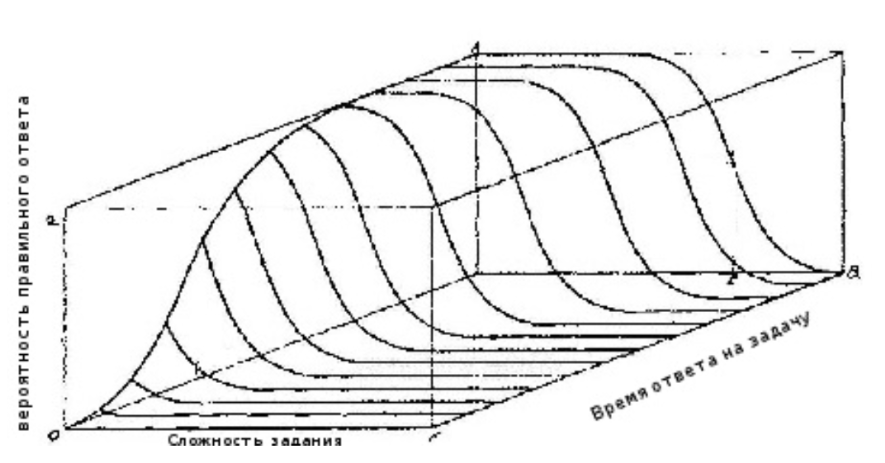
\includegraphics[scale=1]{dSurface.png}}
\end{figure}
Рис. 1.1 Поверхность ответа
\end{center}

	Казалось бы, что данная закономерность проста и понятна, но она также имеет свои недостатки. Во-первых, сама модель исследует только вероятность ответа, а не затраченное на него время. Если сам процесс ответа на задание считать случайным, то обе величины следует рассматривать как случайные и при построении поверхности ответа учитывать их совместное распределение. Также недостатком является и то, что вероятность ответа зависит от двух параметров, сложности задания и способностей тестируемого, но во внимание не принимается время ответа. Кроме того, модель также предполагает зависимость вероятности правильного ответа от времени ответа, однако стандартным предположением в теории ответа на задание является условная независимость между ответами на разные задания одним и тем же студентом.

}

\subsection{Математические модели времени ответа пользователя}{

Несмотря на наличие множества различных моделей, описывающих поведение пользователя во время тестирования, существует всего несколько принципов моделирования времени ответа испытуемого.

Первый принцип моделирования заключается в том, что время ответа и вероятность правильного ответа входят в одно уравнение. В свою очередь он подразделяется на два типа: прямой и обратный. К прямому типу относятся модели ответа, которые включают в себя время, затраченное на ответ, или его параметры. Обратный тип описывает модель времени ответа на задание с помощью самих ответов или их параметров.

Однако типичным для многих моделей IRT является то, что они описывают распределение параметров ответа с использованием параметров характеризующими задания и индивидуальные особенности человека. Введем случайную величину $U_{ij}$, которая может принимать два значения: $U_{ij}=1$, если $j$ - й студент ответил на $i$ - е задание правильно и $U_{ij}=0$ в противном случае. Одной из основных моделей IRT является трехпараметрическая логистическая модель:
\begin{equation}
P\{U_{ij}=1\}=p_i(\theta,a_i,b_i,c_i)\equiv c_i+(1-c_i) \frac{exp[a_i(\theta-b_i)]}{1+exp[a_i(\theta-b_i)]},
\end{equation}
где $\theta$ - способности студента, $b_i$ - сложность задания, $a_i$ - дифференцирующая способность задания, $c_i$ - вероятность угадать ответ на задание.

Примерами прямого типа моделирования являются модели Роскама ([16], [17]), Вана и Хансона [25]. Одна из первых работ принадлежит Роскаму. Его модель представляет собой однопараметрическую логистическую модель ответа с параметром способности студента
\begin{equation}
p_i(\theta_j)={1+exp[-(\theta_j+\ln t_{ij}-b_i)]}^{-1}.
\end{equation}
Для модели справедлива следующая закономерность: при стремлении времени ответа к бесконечности, вероятность правильного ответа приближается к единице. Поэтому она применялась только для тестов на скорость, где неограниченное время ответа почти всегда гарантирует правильный ответ.

Ван и Хансон предложили четырёхпараметрическую логистическую модель ответа
\begin{equation}
p_i(\theta_i)=c_i+(1-c_i){1+exp[-a_i(\theta_j-\rho_j d_i/ t_{ij}-b_i)]}^{-1},
\end{equation}
где $a_i$ - параметр дифференцирующей способности $i$-го задания, $c_i$ - вероятность угадывания ответа для $i$-го задания, $\rho_j$ - параметр медлительности студента, $d_i$ - сложность задания. Основным отличием этой модели от модели Роскама является замена $\ln t_{ij}$ на $-\rho_j d_i/ t_{ij}$. Точность ответа и время ответа моделируются одновременно, но время ответа - независимая переменная, которая влияет на вероятность правильного ответа. С увеличением времени ответа, вероятность правильного ответа приближается к вероятности трехпараметрической логистической модели. По этой причине эта модель применяется к тестам на сложность заданий, где неограниченное время ответа не гарантирует правильного ответа.

К обратному типу моделирования можно отнести работу Тиссена [20]. Его модель применима к тестам на сложность заданий. Тиссен использовал трехпараметрическую логистическую модель для точности ответа и логнормальную модель времени ответа
\begin{equation}
\ln T_{ij}=\mu+\tau_j+\beta_i-\rho(a_i \theta_j-b_i)+\varepsilon_{ij}, \: \varepsilon_{ij}\sim N(0,\sigma^2),
\end{equation}
где $\mu$ - общий параметр для студентов и заданий,  $\tau_j$- медлительность студента, $\beta_i$ -  сложность задания, $\rho$ - регрессионный член параметров $a_i(\theta-b_i)$. Одним из ограничений этой модели  является предположение независимости точности и времени ответа.

Ярким примером второго принципа моделирования является исследование Раша [14] устных тестов на чтение, в котором задействованы два разных типа моделей: первый для количества неправильно прочитанных слов в тексте, второй для скорости чтения. Обе модели основаны на предположении, что чтение является Пуассоновским случайным процессом.

Модель для количества неправильно прочитанных слов в тексте характеризуется числом появления ошибок при прочтении $a$ текста из $N$ слов. Число ошибок при прочтении распределено по закону Пуассона с функцией вероятности вида
\begin{equation}
P(a|N)=e^{-\lambda}\frac{\lambda^a}{a!},
\end{equation}
где $\lambda=N\theta$ - среднее количество ошибок.

Раш определил вероятность $\theta$ как
\begin{equation}
\theta_{ij}=\frac{\delta_i}{\xi_j},
\end{equation}
где $\delta_i$ – сложность $i$–го текста, $\xi_j^{-1}$– навыки $j$–го читателя.

Это простое отношение показывает, что более сложный текст или менее способный читатель имеют большую вероятность допустить ошибку при чтении текста.

Модель для скорости чтения характеризуется временем $t$, необходимым прочтения определенного количества слов. Вероятность того, за заданное время $T$ тестируемый не прочтёт больше $N$ слов, равна значению времени $t$, не превышающего время $T$, необходимое для прочтения $N$ слов. То есть,
\begin{equation}
P(a\geqslant N|T)=P(t\leqslant T|N).
\end{equation}

Время $t$, требующееся для прочтения теста из $N$ слов имеет гамма-распределением с плотностью вероятности вида
\begin{equation}
p(N)=e^{-\lambda t}\frac{(\lambda t)^{N-1}}{(N-1)!},
\end{equation}
где $\lambda$ является параметром интенсивности, характеризующим скорость чтения тестируемого.

Раш также предложил рассматривать параметр скорости $\lambda$ как отношение
\begin{equation}
\lambda_{ij}=\frac{\xi_j}{\delta_i},
\end{equation}
где $\delta_i$ - сложность $i$-го текста, $\xi_j$ - способности $j$-го человека.

Таким образом, обе модели представляют собой пуассоновские потоки.
Совершенно другой подход моделирования представлен в работах В. ван дер Линдена (W. van der Linden, [22,23,24]), которую мы рассмотрим более подробно.
}

\subsection{Модель В. ван дер Линдена}{
В. ван дер Линден [22] предложил двухуровневую иерархическую модель, представленную на рис. 1.2, которая совместно моделирует ответы на задания и время ответа.
На первом уровне расположены вероятностные модели для корректности ответа студента и времени ответа студента. На втором уровне вероятностная модель распределения параметров моделей первого уровня - способность студента и его скорость для студентов всех групп, и вероятностная модель распределения параметров сложности и трудозатрат для каждой задачи из пула.

Время, которое необходимо студенту для выполнения заданий теста и скорость, с которой студент выполняет задания - неэквивалентные понятия. Время ответа студента на задачу может меняться в зависимости от параметров задачи, в то время как скорость студента остаётся неизменной.

\begin{figure}[h]
\center{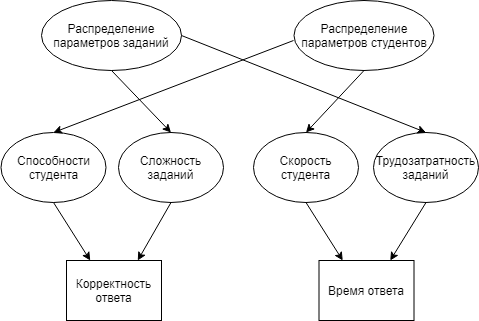
\includegraphics[scale=0.7]{dStructure.png}}
\end{figure}
\begin{center}
Рис. 1.2 Двухуровневая иерархическая модель
\end{center}


Модель Ван дер Линдена предполагает, что логарифм времени ответа \emph{j-}го пользователя на \emph{i-}е задание имеет вид
\begin{equation}
\ln T_{ij}=\mu+\beta_i+\tau_j+\varepsilon_{ij}, \qquad \underset{i=1}{\overset{I}{\sum}}\beta_i=0 , \qquad \underset{j=1}{\overset{J}{\sum}} \tau_j=0,
\end{equation}
%\end{align}
где $T_{ij}$ - случайная величина, обозначающая время ответа $j$-го пользователя на $i$-ю задачу, $\beta_i$ - параметр сложности задания, $\tau_j$ - физиологические особенности пользователя, $\mu$ - общая составляющая для всех пользователей и заданий, $\varepsilon_{ij}$ - случайное отклонение, $\varepsilon_{ij} \sim N(0,\sigma^2), \: i=\overline{1,I}, \:  j=\overline{1,J}$ - независимые гауссовские случайные величины.
Таким образом, время ответа студента на задание имеет логнормальное распределение
\begin{equation}
T_{ij} \sim LogN(\mu+\beta_i+\tau_j,\sigma^2)
\end{equation}
и плотность вероятности вида:
\begin{equation}
f(t_{ij},\mu,\beta_i,\tau_j,\sigma)=\frac{1}{t_{ij} \sqrt{2\pi\sigma^2}} exp \Bigl\{ -\frac{1}{2} \Bigm[\frac{\ln t_{ij}-(\mu+\beta_i+\tau_j)}{\sqrt{\sigma^2}} \Bigm]^2\Bigl\}
\end{equation}

Оценки параметров модели, полученные по методу максимального правдоподобия, были представлены в работе [23]:
\begin{gather}
\hat{\mu}=\frac{ \underset{j=1}{\overset{J}{\sum}} \underset{i=1}{\overset{I}{\sum}} \ln t_{ij}}{IJ}, \\ \hat{\beta_i}=\frac{\underset{j=1}{\overset{J}{\sum}} \ln t_{ij}}{J} - \hat{\mu}, \\
\hat{\tau_j}=\frac{\underset{i=1}{\overset{I}{\sum}} \ln t_{ij}}{I} - \hat{\mu}, \\
\hat{\sigma}^2=\frac{\underset{j=1}{\overset{J}{\sum}} \underset{i=1}{\overset{I}{\sum}} (\ln t_{ij} - \hat{\tau_j} - \hat{\beta_i} - \hat{\mu})^2}{IJ}.
\end{gather}

Эта модель ценна тем, что позволяет получить распределение времени ответа любого пользователя на любое задание системы по имеющейся неполной статистической информации (не все пользователи решали все задачи). Однако существенным недостатком является отсутствие возможности  получить точное значение квантили суммарного времени выполнения теста студентом, которое определяется как сумма логнормальных случайных величин времени ответа пользователя на задания теста.

В работе [1] предлагается преодолеть указанный недостаток использованием гамма-распределения в качестве модели времени ответа пользователя на задание, так как плотности вероятности логнормального и гамма-распределений имеют схожие структуры, и гамма-распределение обладает следующим свойством:\\
Если $\Theta_1,\ldots,\Theta_I$ - независимые СВ, такие что $\Theta_i\sim\Gamma(k_i,\theta), \: i=\overline{1,I},$ то $$\vartheta = \underset{i=1}{\overset{I}{\sum}} \Theta_i \sim \Gamma (\underset{i=1}{\overset{I}{\sum}} k_i,\theta).$$
Необходимо подобрать параметр $\theta$ таким образом, чтобы он был одинаковым для всех задач, и при этом для максимального количества заданий принималась бы гипотеза о гамма-распределении времени ответа пользователя на это задание.

}

\subsection{Алгоритм подбора параметров гамма-распределения}{
Данный алгоритм был представлен в статье [1] для случая, когда в тестировании участвует один универсальный пользователь, однако в случае тестирования группы студентов этот алгоритм требует уточнений.

Пусть в тестировании участвуют $N$ пользователей. Обозначим через $T_i^n$ случайное время, которое потребуется пользователю $n$, на решение $i$ задачи, где $i = \overline{1, I},$ $\: n = \overline{1,N},$ $I$ – число заданий, из которых формируется тест, $\: T_i^n \sim LogN(\hat{\mu}+\hat{\beta}_i+\hat{\tau}_n,\hat{\sigma}^2)$.

Шаг 0. Зафиксировать номер пользователя $n$ и положить $$\theta_n^*=0, k_{in}^*=0, S=0, m=0,$$ где  $\theta_n^*$ - искомое значение параметра гамма-распределения, $k_{in}^*$ - искомое значение второго параметра распределения, $S$ - число задач, для которых принимается гипотеза о гамма-распределении, $m$ - счётчик.

Шаг 1. Для всех $ i=\overline{1,I}$ сгенерировать выборки $t_{in}^\nu$ случайной величины $T^n_i$ объёма $\nu$ и методом максимального правдоподобия найти оценки $\widehat{\theta}_{in}$ параметра $\theta_n$. Положить

$$\widehat{\theta}_{min\; n}=\underset{i=\overline{1,I}}{\overset{}{ min}}\{\widehat{\theta}_{in}\},\;
\widehat{\theta}_{max\;n}=\underset{i=\overline{1,I}}{\overset{}{ max}}\{\widehat{\theta}_{in}\},$$
$$h=\frac{\widehat{\theta}_{max\;n}-\widehat{\theta}_{min\;n}}{L}, \: \theta^m_{n}=\widehat{\theta}_{min\;n}-h,$$
где $h$ - шаг для варьирования $\theta_n$, $L$ - число шагов дискретизации.

Шаг 2. Положить $m:=m+1, \theta^m_{n}=\theta^{m-1}_{n}+h$. Для каждого $i=\overline{1,I}$ по выборке $t_{in}^\nu$ определить оценку второго параметра
$$\widehat{k}_{in}=\frac{\overline{t}_{in}^\nu}{\theta^m_{n}},$$
где $\overline{t}_{in}^\nu$ - выборочное математическое ожидание.

Шаг 3. Для всех $ i=\overline{1,I}$ проверить гипотезу $H_0=t_{in}\sim\Gamma(\widehat{k}_{in},\theta^m_{n})$ с помощью критерия Пирсона на выбранном уровне доверительной вероятности $1-\alpha$. Если число принятых гипотез $S'>S$, то положить $S=S', \theta_n^*=\theta^m_{n}, k^*_{in}=\widehat{k}_{in}, i=\overline{1,I}.$

Шаг 4. Если $m\leqslant L-1,$ то перейти к шагу 2.

Шаг 5. Окончание работы алгоритма.


}

\subsection{Постановка задачи поиска наборов заданий для проведения ограниченного по времени тестирования}{
Задача определения некоторого набора приблизительно равных по суммарной сложности заданий была рассмотрена в [5,8] и выглядит следующим
образом.

Пусть существует множество $Z = (z_1,\ldots, z_I)$ из $I$ заданий, разделенных на $M$ различных типов, $I_m$ - число заданий $m$-го типа, тогда $\underset{m=1}{\overset{M}{\sum}} I_m = I$, $m = \overline{1,M}.$ Для обозначения принадлежности задания к определенному типу введем матрицу $A$ размерности $I\times M$:
\[
A =\parallel a_i^m\parallel, a_i^m =
\begin{cases}
1, & \text{$z_i\in Z_m$,} \\
0, & \text{$z_i\notin Z_m$.}
\end{cases}
\]

Пусть $u \in R^I$ вектор принадлежности задания к тесту:
$$
u_i =
\begin{cases}
1, & \text{если задача $i$ попала в тестовый набор,} \\
0, & \text{если задача $i$ не попала в тестовый набор.}
\end{cases}
$$

Каждое из заданий имеет определенную различную сложность, которую, например, можно определить с помощью метода максимального
правдоподобия, примененного к модели Раша в [14]. Определим вектор $w \in R^I$, $i$-я координата которого является сложностью $i$-го задания.

Требуется составить множество тестовых наборов из $k$ заданий, принадлежащим различным типам, учитывая, что количество заданий в тесте должно быть больше или равно количеству типов заданий, то есть $k\geqslant M$. При этом изначально задаётся суммарная сложность теста $c$ и предусматривается возможность отклонения подобранного набора заданий на какое-либо маленькое число $\varepsilon$.

Пусть по-прежнему в тестировании участвуют $N$ пользователей, $T_i^n$ случайное время, необходимое пользователю $n$ на решение $i$ - й задачи, $i = \overline{1, I},$ $\: n = \overline{1,N},$ $\: T_i^n \sim LogN(\hat{\mu}+\hat{\beta}_i+\hat{\tau}_n,\hat{\sigma}^2)$. Рассмотрим матрицу $T$ размерности $N \times I$:
$$T = \parallel T^n_i\parallel.$$
Будем предполагать, что случайные величины $T^n_i$ являются независимыми.

Пусть в отличие от модели, полученной в [5], общее время на выполнение теста неизвестно, аналогично [1,8]. Обозначим его через $\varphi$. Тогда для того, чтобы за некоторое оптимальное время все тестируемые могли выполнить выданный вариант теста с заданной вероятностью $\alpha$, рассмотрим функцию квантили:
\begin{gather}
\Phi_\alpha (u) {\overset{\triangle}{=}} min\{\varphi \in R^1: P\{\underset{n=\overline{1,N}}{\overset{}{max}} T_n u\leqslant\varphi\}\geqslant\alpha\},
\end{gather}
где $ T_n,\: n-$я строка матрицы $T$.

После перехода к гамма-распределению времени ответа пользователей с помощью алгоритма, описанного в разделе 1.6, в предположении, что случайные величины являются независимыми, функция квантили в (1.18) примет вид:
\begin{gather}
\Phi_\alpha (u) {\overset{\triangle}{=}} min\{\varphi \in R^1: P\{\underset{n=\overline{1,N}}{\overset{}{max}} \Theta_n u\leqslant\varphi\}\geqslant\alpha\},
\end{gather}
где $\Theta_i^n \sim \Gamma(\hat{k}_{in},\hat{\theta}_n)$, $\Theta^n_i$ - случайное время, которое потребуется пользователю $n$ на решение $i$ задачи, $ \Theta = \parallel \Theta^n_i\parallel$ - матрица размерности $N \times I$,  $ \Theta_n$ - $n$-я строка матрицы $\Theta$.

В силу свойств гамма-распределения, её можно записать в виде:
\begin{equation}
    \begin{split}
        \Phi_\alpha (u) &{\overset{\triangle}{=}} min\{\varphi \in R^1: P\{\vartheta_1\leqslant\varphi,\ldots,\vartheta_N\leqslant\varphi\}\geqslant\alpha\} =\\
        &= min\{\varphi \in R^1: F_{\vartheta_1}(\varphi)\cdot\ldots\cdot F_{\vartheta_N}(\varphi)\geqslant\alpha\},
    \end{split}
\end{equation}
где $\vartheta_n=\Theta_n\cdot u,\; \vartheta_n\sim\Gamma(\hat{k}_n^T\cdot u,\; \hat{\theta}_n), \; n=\overline{1,N}$ - независимые случайные величины, $\hat{k}_n=(\hat{k}_{1n}, \ldots, \hat{k}_{In})^T,\; n=\overline{1,N}.$

Основываясь на описанной модели и введенных обозначениях, сформулируем задачу квантильной оптимизации:

\begin{gather}
u_\alpha=Arg \:\underset{u\in \{0,1\}^I}{\overset{}{ min}}\:(\gamma\frac{\mid c-w^T u \mid}{\varepsilon} + (1-\gamma)\frac{\Phi_\alpha(u)}{2700}),\\
\varphi_\alpha=\underset{u\in \{0,1\}^I}{\overset{}{min}}\:(\gamma\frac{\mid c-w^T u \mid}{\varepsilon} + (1-\gamma)\frac{\Phi_\alpha(u)}{2700}),\\
c-w^T u\leqslant\varepsilon, \\
w^T u-c\leqslant\varepsilon, \\
A^Tu\geqslant e_M, \\
e^Tu=k,
\end{gather}
где $(\cdot)^T$ - операция транспонирования,\: $\gamma\in[0,1]$ - весовой коэффициент,\: $\alpha\in(0,1)$  - заданный уровень доверительной вероятности, $e=(1,\ldots,1)^T$, $e \in R^I$, $e_M=(1,\ldots,1)^T,\: e_M \in R^M$.

Функция (1.21) является критериальной в исследуемой задаче. Она представляет из себя сумму двух нормированных безразмерных величин. Первое слагаемое является отклонением сложности теста от заданного уровня $c$, нормированного максимально допустимым уровнем отклонения $\varepsilon$. Второе слагаемое представляет из себя время выполнения теста, которое не может быть превышено с заданным уровнем доверительной вероятности $\alpha$. Это время нормируется максимально допустимым временем выполнения теста. Такой критерий представляется универсальным гибким инструментом формирования теста. С помощью весового аргумента $\gamma\in[0,1]$ можно регулировать важность каждого слагаемого. Ограничения (1.23) и (1.24) обозначают границы выбора набора заданий в тесте в зависимости от отклонения от требуемой суммарной сложности. Ограничение (1.25) отвечает за то, чтобы среди всех заданий в тесте было хотя бы одно задание каждого типа, так как данная задача решается при условии, что $k \geqslant M$. Ограничение (1.26) означает, что в наборе должно быть ровно $k$ заданий.

%В данной постановке присутствует весовой коэффициент $\gamma\in[0,1]$, который позволяет сделать акцент либо на минимизации отклонения сложности подобранного набора заданий в тесте $w^T u$ от требуемой сложности $c$, либо на минимизации времени ответа пользователя. Функция (1.22) обозначает оптимальное значение времени ответа пользователя.
}

\newpage
\headsep=12cm
\begin{center} \section{ПРАКТИЧЕСКАЯ ЧАСТЬ} \end{center}

\headsep=25pt

\subsection{Алгоритм поиска оптимального набора заданий}{

Сформулированная одноэтапная задача стохастического программирования с квантильным критерием имеет достаточно большую размерность. Для её решения предлагается декомпозиционный алгоритм, позволяющий существенно сократить количество вычислительных операций.

Шаг 1. Составить множество $\overline{U}$ всех $u$, удовлетворяющих неравенствам (1.23) - (1.26): $$\overline{U} \underset{}{\overset{\triangle}{=}} \{ u \in R^I : c-w^T u\leqslant\varepsilon, \: w^T u-c\leqslant\varepsilon, \: A^Tu\geqslant e_M, \: e^Tu=k, \: u \in \{0,1\}^I \}; $$

Шаг 2. Для каждого $u^s \in \overline{U}$ найти
$$\varphi_{s}^{\ast}\triangleq min \{ \varphi \in R^1: F_{\vartheta_1}(\varphi)\cdot\ldots\cdot F_{\vartheta_N}(\varphi)\geqslant\alpha\},\; n=1,\ldots,N,$$
$$ \psi_s^\ast=\gamma \frac{\mid c-w^T u^s \mid}{\varepsilon}  + (1-\gamma)\frac{\varphi_s^\ast}{2700}$$

Шаг 3. Среди всех $\psi_s^\ast$ выбираем наименьшее ($\psi_{s^\ast}^\ast$);

Шаг 4. Полагаем решение исходной задачи (1.20)-(1.26) равным $u^{s^\ast},\psi_{s^\ast}^\ast,\varphi_{s^\ast}^\ast$.
}

\subsection{Численный эксперимент}{
Для проведения анализа сформулируем задачу, исходные данные которой получены при обработке статистической информации системы дистанционного обучения МАИ CLASS.NET в [5].

Рассмотрим задания M = 3 различных типов, относящихся к основным изучаемым в течение первого семестра тематическим разделам курса по «Математическому анализу» СДО МАИ CLASS.NET, в каждом из которых по 10 различных заданий $I_m=10, \: m=1, \cdots, 3$. Обозначим задания в зависимости от типа $m=1, \cdots, M$ и номера $i=1, \cdots, I_m$ как $z_i^m$. В [9] была проведена оценка сложности каждого задания из общего количества при помощи алгоритма, основанного на модели Раша. В результате были получены приведенные к десятибалльной шкале оценки значений сложностей $w_i^m$ для каждого задания $z_i^m$, которые представлены в таблице 2.1.

\begin{table}[h!]
\centering
\begin{flushright}
Таблица 2.1 Сложность $w_i^m$ задания $z_i^m$
\end{flushright}
\begin{tabular}{|>{\centering}m{22pt}|>{\centering}m{31pt}|>{\centering}m{31pt}|>{\centering}m{31pt}|>{\centering}m{31pt}|>{\centering}m{31pt}|>{\centering}m{31pt}|>{\centering}m{31pt}|>{\centering}m{31pt}|>{\centering}m{31pt}|c|}
\hline
$m\backslash i$ &1 	& 2 	& 3 	& 4 	& 5 	& 6 	& 7 	& 8 	& 9 	& 10 \\ \hline
1 	&1.311 &3.254 & 3.254 & 3.254 & 4.874 & 5.368 & 7.011 & 7.217 & 8.244 & 9.636 \\ \hline
2 	&4.132 &6.902 & 2.121 & 3.436 & 2.456 & 5.359 & 6.902 & 7.283 & 7.815 & 9.399 \\ \hline
3 	&2 	&2.418 & 2.666 & 3.653 & 5.242 & 5.547 & 6.453 & 7.194 & 8.795 & 3.657 \\ \hline
\end{tabular}
\label{ch2}
\end{table}

Исходя из оценок значений сложности для каждого задания, выберем требуемую суммарную сложность $c = 29.46$ теста из $k = 5$, возможный критерий выбора которой был описан в [5,8], и параметр отклонений от требуемой суммарной сложности $\varepsilon$. Параметр $\varepsilon$ задается числом, близким к нулю, для выбора наиболее оптимальных наборов тестов. Будем варьировать его от $0.001$ до $0.005$ с шагом $0.001$. Далее будем подбирать тест из 5 заданий для группы из $N=3$ студентов. Для каждого задания и каждого студента были получены оценки значений параметров логнормального распределения, которые приведены в таблицах 2.2, 2.3 и 2.4.

\begin{table}[h!]
\centering
\begin{flushright}
Таблица 2.2 Значения параметров логнормального распределения случайных величин $T_i^1 \sim LogN(\hat{\mu}+\hat{\beta}_i^m+\hat{\tau}_1,0.31)$
\end{flushright}
\begin{tabular}{|>{\centering}m{60pt}|c|>{\centering}m{60pt}|c|>{\centering}m{60pt}|c|}
\hline
$z_i^m$ 	&$\hat{\mu}+\hat{\beta}_i^m+\hat{\tau}_1$ & $z_i^m$	& $\hat{\mu}+\hat{\beta}_i^m+\hat{\tau}_1$ & $z_i^m$ & $\hat{\mu}+\hat{\beta}_i^m+\hat{\tau}_1$ \\ \hline
$z_1^1$		& 3.6749							  & $z_1^2$	& 4.4811							   & $z_1^3$ & 5.2252 \\ \hline
$z_2^1$		& 3.7349							  & $z_2^2$	& 4.5123							   & $z_2^3$ & 5.3832 \\ \hline
$z_3^1$		& 3.9170							  & $z_3^2$	& 4.6278							   & $z_3^3$ & 5.3917 \\ \hline
$z_4^1$		& 3.9813							  & $z_4^2$	& 4.6957							   & $z_4^3$ & 5.4756 \\ \hline
\end{tabular}
\label{ch2}
\end{table}

\begin{table}[h!]
\centering
\begin{flushright}
Продолжение таблицы 2.2
\end{flushright}
\begin{tabular}{|>{\centering}m{57pt}|c|>{\centering}m{57pt}|c|>{\centering}m{57pt}|c|}
\hline
$z_i^m$ 	&$\hat{\mu}+\hat{\beta}_i^m+\hat{\tau}_1$ & $z_i^m$	& $\hat{\mu}+\hat{\beta}_i^m+\hat{\tau}_1$ & $z_i^m$ & $\hat{\mu}+\hat{\beta}_i^m+\hat{\tau}_1$ \\ \hline
$z_5^1$		& 4.0064							  & $z_5^2$	& 4.8405							   & $z_5^3$ & 6.0034 \\ \hline
$z_6^1$		& 4.1700							  & $z_6^2$	& 4.9326							   & $z_6^3$ & 6.0279 \\ \hline
$z_7^1$		& 4.2830							  & $z_7^2$	& 5.0219							   & $z_7^3$ & 6.0547 \\ \hline
$z_8^1$		& 4.3145							  & $z_8^2$	& 5.0329							   & $z_8^3$ & 6.0760 \\ \hline
$z_9^1$		& 4.3420							  & $z_9^2$	& 5.0844							   & $z_9^3$ & 6.0955 \\ \hline
$z_{10}^1$	& 4.3478							  & $z_{10}^2$	& 5.1582						   & $z_{10}^3$	& 6.1444 \\ \hline
\end{tabular}
\label{ch2}
\end{table}

\begin{table}[h!]
\centering
\begin{flushright}
Таблица 2.3 Значения параметров логнормального распределения случайных величин $T_i^2 \sim LogN(\hat{\mu}+\hat{\beta}_i^m+\hat{\tau}_2,0.31)$
\end{flushright}
\begin{tabular}{|>{\centering}m{60pt}|c|>{\centering}m{60pt}|c|>{\centering}m{60pt}|c|}
\hline
$z_i^m$ 	&$\hat{\mu}+\hat{\beta}_i^m+\hat{\tau}_2$ & $z_i^m$	& $\hat{\mu}+\hat{\beta}_i^m+\hat{\tau}_2$ & $z_i^m$ & $\hat{\mu}+\hat{\beta}_i+\hat{\tau}_2$ \\ \hline	
$z_1^1$		& 3.7228	& $z_1^2$	& 4.5863	& $z_1^3$	& 5.9014 \\ \hline
$z_2^1$		& 3.7324	& $z_2^2$	& 4.7554	& $z_2^3$	& 5.9762 \\ \hline
$z_3^1$		& 3.9238	& $z_3^2$	& 5.0698	& $z_3^3$	& 6.0362 \\ \hline
$z_4^1$		& 4.0022	& $z_4^2$	& 5.2120	& $z_4^3$	& 6.2504 \\ \hline
$z_5^1$		& 4.0183	& $z_5^2$	& 5.3798	& $z_5^3$	& 6.2885 \\ \hline
$z_6^1$		& 4.2069	& $z_6^2$	& 5.4517	& $z_6^3$	& 6.3291 \\ \hline
$z_7^1$		& 4.4406	& $z_7^2$	& 5.4526	& $z_7^3$	& 6.4350 \\ \hline
$z_8^1$		& 4.4525	& $z_8^2$	& 5.5283	& $z_8^3$	& 6.4756 \\ \hline
$z_9^1$		& 4.4591	& $z_9^2$	& 5.5619	& $z_9^3$	& 6.5154 \\ \hline
$z_{10}^1$	& 4.5748	& $z_{10}^2$& 5.8704	& $z_{10}^3$& 6.5224 \\ \hline
\end{tabular}
\label{ch2}
\end{table}

\begin{table}[h!]
\centering
\begin{flushright}
Таблица 2.4 Значения параметров логнормального распределения случайных величин $T_i^3 \sim LogN(\hat{\mu}+\hat{\beta}_i^m+\hat{\tau}_3,0.31)$
\end{flushright}
\begin{tabular}{|>{\centering}m{57pt}|c|>{\centering}m{57pt}|c|>{\centering}m{57pt}|c|}
\hline
$z_i^m$ 	&$\hat{\mu}+\hat{\beta}_i^m+\hat{\tau}_3$ & $z_i^m$	& $\hat{\mu}+\hat{\beta}_i^m+\hat{\tau}_3$ & $z_i^m$ & $\hat{\mu}+\hat{\beta}_i^m+\hat{\tau}_3$	\\ \hline
$z_1^1$		& 3.6065	& $z_1^2$		& 4.6182	& $z_1^3$		& 5.5426 \\ \hline
$z_2^1$		& 3.6466	& $z_2^2$		& 4.7260	& $z_2^3$		& 5.6243 \\ \hline
$z_3^1$		& 3.7396	& $z_3^2$		& 4.7377	& $z_3^3$		& 5.6503 \\ \hline
$z_4^1$		& 3.7407	& $z_4^2$		& 4.7604	& $z_4^3$		& 5.6801 \\ \hline
$z_5^1$		& 4.0330	& $z_5^2$		& 4.9201	& $z_5^3$		& 5.7959 \\ \hline
$z_6^1$		& 4.0605	& $z_6^2$		& 4.9586	& $z_6^3$		& 5.8392 \\ \hline
$z_7^1$		& 4.2256	& $z_7^2$		& 5.0281	& $z_7^3$		& 5.9118 \\ \hline
$z_8^1$		& 4.3427	& $z_8^2$		& 5.2476	& $z_8^3$		& 5.9979 \\ \hline
$z_9^1$		& 4.4738	& $z_9^2$		& 5.3011	& $z_9^3$		& 6.1737 \\ \hline
$z_{10}^1$	& 4.4882	& $z_{10}^2$	& 5.4072	& $z_{10}^3$	& 6.1785 \\ \hline
\end{tabular}
\label{ch2}
\end{table}

С помощью алгоритма, описанного в главе 1.6,  для каждого студента и каждого задания были получены оценки параметров гамма-распределения. Эти значения представлены в таблицах 2.5, 2.6 и 2.7.
\newpage

\begin{table}[h!]
\centering
\begin{flushright}
Таблица 2.5 Значения параметров гамма-распределения \\ случайных величин $\Theta_i^1 \sim \Gamma(\hat{k}_{i1}^m,2.0362)$
\end{flushright}
\begin{tabular}{|>{\centering}m{60pt}|>{\centering}m{70pt}|>{\centering}m{60pt}|>{\centering}m{70pt}|>{\centering}m{60pt}|>{\centering\arraybackslash}m{70pt}|}
\hline
$z_i^m$ 	& $\hat{k}_{i1}^m$	& $z_i^m$ 	& $\hat{k}_{i1}^m$  &$z_i^m$ 	& $\hat{k}_{i1}^m$ \\ \hline
$z_1^1$		& 24.1437	& $z_1^2$	& 54.4736	& $z_1^3$	& 108.1962 \\ \hline
$z_2^1$		& 24.5458	& $z_2^2$	& 56.4882	& $z_2^3$	& 125.0120 \\ \hline
$z_3^1$		& 30.1015	& $z_3^2$	& 62.1900	& $z_3^3$	& 139.8069 \\ \hline
$z_4^1$		& 32.7089	& $z_4^2$	& 66.2862	& $z_4^3$	& 146.9207 \\ \hline
$z_5^1$		& 32.2862	& $z_5^2$	& 74.4638	& $z_5^3$	& 236.1203 \\ \hline
$z_6^1$		& 40.1710	& $z_6^2$	& 83.9135	& $z_6^3$	& 239.7240 \\ \hline
$z_7^1$		& 43.8352	& $z_7^2$	& 87.0075	& $z_7^3$	& 260.1843 \\ \hline
$z_8^1$		& 44.4992	& $z_8^2$	& 90.8004	& $z_8^3$	& 258.5974 \\ \hline
$z_9^1$		& 46.3532	& $z_9^2$	& 98.7714	& $z_9^3$	& 251.3356 \\ \hline
\end{tabular}
\label{ch2}
\end{table}

\begin{table}[h!]
\centering
\begin{flushright}
Продолжение таблицы 2.5
\end{flushright}
\begin{tabular}{|>{\centering}m{60pt}|>{\centering}m{70pt}|>{\centering}m{60pt}|>{\centering}m{70pt}|>{\centering}m{60pt}|>{\centering\arraybackslash}m{70pt}|}
\hline
$z_i^m$ 	& $\hat{k}_{i1}^m$	& $z_i^m$ 	& $\hat{k}_{i1}^m$  &$z_i^m$ 	& $\hat{k}_{i1}^m$ \\ \hline

$z_{10}^1$	& 49.6794	& $z_{10}^2$& 106.2339	& $z_{10}^3$& 290.0428 \\ \hline
\end{tabular}
\label{ch2}
\end{table}


\begin{table}[h!]
\centering
\begin{flushright}	
Таблица 2.6 Значения параметров гамма-распределения случайных величин $\Theta_i^2 \sim \Gamma(\hat{k}_{i2}^m,2.4018)$
\end{flushright}
\begin{tabular}{|>{\centering}m{60pt}|>{\centering}m{70pt}|>{\centering}m{60pt}|>{\centering}m{70pt}|>{\centering}m{60pt}|>{\centering\arraybackslash}m{70pt}|}
\hline
$z_i^m$ 	& $\hat{k}_{i2}^m$	&$z_i^m$ 	& $\hat{k}_{i2}^m$	& $z_i^m$ 	& $\hat{k}_{i2}^m$ 	\\ \hline		
$z_1^1$		& 21.1209	& $z_1^2$		& 49.1616		& $z_1^3$		& 187.9989	\\ \hline
$z_2^1$		& 21.0962	& $z_2^2$		& 58.0855		& $z_2^3$		& 196.5221	\\ \hline
$z_3^1$		& 26.8960	& $z_3^2$		& 80.8067		& $z_3^3$		& 210.2317	\\ \hline
$z_4^1$		& 28.8030	& $z_4^2$		& 89.3256		& $z_4^3$		& 260.2312	\\ \hline
$z_5^1$		& 26.9206	& $z_5^2$		& 106.4342		& $z_5^3$		& 280.4852	\\ \hline
$z_6^1$		& 33.0081	& $z_6^2$		& 120.6380		& $z_6^3$		& 287.2276	\\ \hline
$z_7^1$		& 44.0495	& $z_7^2$		& 115.3710		& $z_7^3$		& 305.4095	\\ \hline
$z_8^1$		& 44.5630	& $z_8^2$		& 135.5043		& $z_8^3$		& 326.1914	\\ \hline
$z_9^1$		& 44.6061	& $z_9^2$		& 131.7241		& $z_9^3$		& 331.9568	\\ \hline
$z_{10}^1$	& 50.2366	& $z_{10}^2$	& 169.0295		& $z_{10}^3$	& 358.9178	\\ \hline
\end{tabular}
\label{ch2}
\end{table}

\begin{table}[h!]
\centering
\begin{flushright}
Таблица 2.7 Значения параметров гамма-распределения случайных величин $\Theta_i^3 \sim \Gamma(\hat{k}^m_{i3},1.7742)$	
\end{flushright}
\begin{tabular}{|>{\centering}m{60pt}|>{\centering}m{70pt}|>{\centering}m{60pt}|>{\centering}m{70pt}|>{\centering}m{60pt}|>{\centering\arraybackslash}m{70pt}|}
\hline
$z_i^m$ 	& $\hat{k}_{i3}^m$	& $z_i^m$ 	& $\hat{k}_{i3}^m$	& $z_i^m$ 	& $\hat{k}_{i3}^m$ \\ \hline						
$z_1^1$		& 24.5770	& $z_1^2$		& 66.0086		& $z_1^3$		& 168.2970 	\\ \hline
$z_2^1$		& 27.6303	& $z_2^2$		& 77.3029		& $z_2^3$		& 189.5198 	\\ \hline
$z_3^1$		& 30.7030	& $z_3^2$		& 78.2095		& $z_3^3$		& 195.6702 	\\ \hline
$z_4^1$		& 28.4557	& $z_4^2$		& 80.1137		& $z_4^3$		& 201.7689 	\\ \hline
$z_5^1$		& 39.7783	& $z_5^2$		& 91.3975		& $z_5^3$		& 232.5395 	\\ \hline
\end{tabular}
\label{ch2}
\end{table}

\begin{table}[h!]
\centering
\begin{flushright}
Продолжение таблицы 2.7
\end{flushright}
\begin{tabular}{|>{\centering}m{60pt}|>{\centering}m{70pt}|>{\centering}m{60pt}|>{\centering}m{70pt}|>{\centering}m{60pt}|>{\centering\arraybackslash}m{70pt}|}
\hline
$z_i^m$ 	& $\hat{k}_{i3}^m$	& $z_i^m$ 	& $\hat{k}_{i3}^m$	& $z_i^m$ 	& $\hat{k}_{i3}^m$ \\ \hline	
$z_6^1$		& 39.8163	& $z_6^2$		& 93.2873		& $z_6^3$		& 219.7571 	\\ \hline
$z_7^1$		& 48.3405	& $z_7^2$		& 100.8703		& $z_7^3$		& 253.2464 	\\ \hline
$z_8^1$		& 53.1551	& $z_8^2$		& 124.9839		& $z_8^3$		& 279.6308 	\\ \hline
$z_9^1$		& 58.0723	& $z_9^2$		& 142.9349		& $z_9^3$		& 335.7254 	\\ \hline
$z_{10}^1$	& 61.3711	& $z_{10}^2$	& 155.6476		& $z_{10}^3$	& 328.6116 	\\ \hline
\end{tabular}
\label{ch2}
\end{table}

На уровне доверительной вероятности 0.95 критерий Пирсона показал, что все гипотезы о том, что время ответа всех трёх пользователей на соответствующие задания системы имеет гамма-распределение с указанными параметрами, принимаются. Для каждого набора заданий $u\in\overline{U}$ с помощью критерия хи-квадрат Пирсона была проверена и принята гипотеза о независимости случайных величин $\vartheta_n\sim\Gamma(\hat{k}_n^T\cdot u,\hat{\theta}_n),n=\overline{1,3}$.

Требовалось составить наборы тестовых заданий из 5 задач, которые с вероятностью 0.95 могли быть решены 3-мя студентами за некоторое оптимальное время $\varphi$. Для каждого $\varepsilon$ были получены наборы заданий, удовлетворяющие детерминированным ограничениям.
Среди каждого такого набора был выбран тест, для которого значение критериальной функции оказалось минимальным. При решении задачи весовой коэффициент $\gamma$ варьировался от 0 до 1 с шагом 0.1. Основные результаты вычислений для $\gamma=0,\:\gamma=0.5$ и $\gamma=1$ представлены в таблицах 2.8, 2.9 и 2.10. Эти значения выбраны неслучайно, при $\gamma=0$ в задаче (1.20) - (1.26) минимизируется время ответа пользователя, при $\gamma=1$, напротив, минимизируется отклонение сложности подобранного теста от требуемой суммарной сложности, а при $\gamma=0.5$ слагаемые в критериальной функции имеют равный вес. Как видно из таблиц, итоговые наборы заданий в тесте различны для каждого из этих значений весового коэффициента $\gamma$.
%, а также получены результаты для различных значений $\gamma=0,\: \gamma=0.5$ и $\gamma=1$ для этих наборов (таблица 2.3). Как видно из результата, для случая, когда минимизация отклонения сложности набора тестовых заданий и минимизация оптимального времени ответа имеют равный вес, приоритет всё же отдается минимизации отклонения, так как с увеличением 𝜀 оптимальный набор заданий не изменяется
%Как видно из таблицы 1, при увеличении отклонения эпсилон количество наборов заданий, удовлетворяющих детерминированным ограничениям, растёт.

\begin{table}[h!]
\centering
\begin{flushright}
Таблица 2.8 Подбор оптимального набора заданий при $\gamma=0$
\end{flushright}
\begin{tabular}{|c|c|c|c|c|}
\hline
            	& Количество        & \multicolumn{3}{c|}{$\gamma = 0$}	                        					 \\ \cline{3-5}
				& решений,          & \multirow{4}{80pt}{\centering{Значение квантили $\varphi^\ast$ (минуты)}}	&\multirow{4}{60pt}{\centering{Значение критерия $\psi^\ast$}} &   			 \\
$\varepsilon$	& удовлетворяющих	&               &       				& Номера заданий,						 \\
				& детерминированным	&               &       				& вошедших в тест  						 \\
				& ограничениям		&       		&           			&                 						 \\ \cline{1-5}
0.001			& 7			        & 23.3651 		& 0.5192				& $z^1_6, z^2_1, z^2_2, z^2_9, z^3_5$	 \\ \cline{1-5}		
0.002			& 21		        & 23.3651		& 0.5192				& $z^1_6, z^2_1, z^2_2, z^2_9, z^3_5$    \\ \cline{1-5}
0.003			& 30		        & 22.0362		& 0.4897				& $z^1_7, z^1_{10}, z^2_1, z^2_4, z^3_5$ \\ \cline{1-5}					
0.004			& 35		        & 22.0362		& 0.4897				& $z^1_7, z^1_{10}, z^2_1, z^2_4, z^3_5$ \\ \cline{1-5}			
0.005			& 40		        & 22.0362		& 0.4897				& $z^1_7, z^1_{10}, z^2_1, z^2_4, z^3_5$ \\ \cline{1-5}	
\end{tabular}
\label{ch2}
\end{table}


\begin{table}[h!]
\centering
\begin{flushright}
Таблица 2.9 Подбор оптимального набора заданий при $\gamma=0.5$
\end{flushright}
\begin{tabular}{|c|c|c|c|c|}
\hline
            	& Количество        & \multicolumn{3}{c|}{$\gamma = 0.5$}	                        					 \\ \cline{3-5}
				& решений,          & \multirow{4}{80pt}{\centering{Значение квантили $\varphi^\ast$ (минуты)}}	&\multirow{4}{60pt}{\centering{Значение критерия $\psi^\ast$}} &   			 \\
$\varepsilon$	& удовлетворяющих	&               &       				& Номера заданий,						 \\
				& детерминированным	&               &       				& вошедших в тест  						 \\
				& ограничениям		&       		&           			&                 						 \\ \cline{1-5}
0.001			& 7			        & 33.5329		& 0.5226				& $z^1_6, z^1_{10}, z^2_5, z^3_6, z^3_7	$ \\ \cline{1-5}
0.002			& 21		        & 33.5329		& 0.5226				& $z^1_6, z^1_{10}, z^2_5, z^3_6, z^3_7	$ \\ \cline{1-5}
0.003			& 30		        & 23.3651		& 0.3929        		& $z^1_6, z^2_1, z^2_2, z^2_9, z^3_5$	  \\ \cline{1-5}
0.004			& 35		        & 23.3651		& 0.3929        		& $z^1_6, z^2_1, z^2_2, z^2_9, z^3_5$     \\ \cline{1-5}
0.005			& 40		        & 23.3651		& 0.3929        		& $z^1_6, z^2_1, z^2_2, z^2_9, z^3_5$	  \\ \cline{1-5}
\end{tabular}
\label{ch2}
\end{table}

Наибольшему количеству наборов заданий соответствует $\varepsilon=0.005$, для этого значения $\varepsilon$ в таблице 2.11 приведено подробное исследование влияния значения весового коэффициента $\gamma$ на подбор теста. Можно заметить, что при увеличении значения $\gamma$ отклонение сложности подобранного теста от заданной уменьшается, а время выполнения теста растёт. Для более наглядного анализа изменения времени выполнения, эти же результаты представлены на рисунке 2.1. Цветом выделены тестовые наборы заданий, одному тесту соответствует один цвет.

\begin{table}[h!]
\centering
\begin{flushright}
Таблица 2.10 Подбор оптимального набора заданий при $\gamma=1$
\end{flushright}
\begin{tabular}{|c|c|c|c|c|}
\hline
            	& Количество        & \multicolumn{3}{c|}{$\gamma = 1$}	                        					 \\ \cline{3-5}
				& решений,          & \multirow{4}{80pt}{\centering{Значение квантили $\varphi^\ast$ (минуты)}}	&\multirow{4}{60pt}{\centering{Значение критерия $\psi^\ast$}} &   			 \\
$\varepsilon$	& удовлетворяющих	&               &       				& Номера заданий,						 \\
				& детерминированным	&               &       				& вошедших в тест  						 \\
				& ограничениям		&       		&           			&                 						 \\ \cline{1-5}
\multirow{2}*{0.001}	& \multirow{2}*{7}		& 34.7905		& 0.3000		& $z^1_5, z^1_8, z^2_3, z^3_7, z^3_9$	  	\\ \cline{3-5}
						&						& 33.5329		& 0.3000 		& $z^1_6, z^1_{10}, z^2_5, z^3_6, z^3_7	$	\\ \cline{1-5}
\multirow{2}*{0.002}	& \multirow{2}*{21}		& 34.7905		& 0.1500 		& $z^1_5, z^1_8, z^2_3, z^3_7, z^3_9$		\\ \cline{3-5}
						&						& 33.5329		& 0.1500 		& $z^1_6, z^1_{10}, z^2_5, z^3_6, z^3_7$	\\ \cline{1-5}
\multirow{2}*{0.003}	& \multirow{2}*{30}		& 34.7905		& 0.1000		& $z^1_5, z^1_8, z^2_3, z^3_7, z^3_9$		\\ \cline{3-5}		
						&						& 33.5329		& 0.1000		& $z^1_6, z^1_{10}, z^2_5, z^3_6, z^3_7$	\\ \cline{1-5}
\multirow{2}*{0.004}	& \multirow{2}*{35}		& 34.7905		& 0.0750		& $z^1_5, z^1_8, z^2_3, z^3_7, z^3_9$ 		\\ \cline{3-5}
						&						& 33.5329		& 0.0750		& $z^1_6, z^1_{10}, z^2_5, z^3_6, z^3_7$	\\ \cline{1-5}			
\multirow{2}*{0.005}	& \multirow{2}*{40}		& 34.7905		& 0.0600		& $z^1_5, z^1_8, z^2_3, z^3_7, z^3_9$		\\ \cline{3-5}
						& 						& 33.5329		& 0.0600		& $z^1_6, z^1_{10}, z^2_5, z^3_6, z^3_7$	\\ \cline{1-5}			
\end{tabular}
\label{ch2}
\end{table}

\begin{table}[h!]
\centering
\begin{flushright}
Таблица 2.11 Подбор оптимального набора заданий для $\varepsilon=0.005$ и различных значений весового коэффициента $\gamma$
\end{flushright}
\begin{tabular}{|>{\centering}m{30pt}|c|c|c|c|c|}
\hline
			&Значение  						   &Значение   				&Оптимальный&				  &Значение \\
$\gamma$	&квантили $\varphi^\ast$           &квантили $\varphi^\ast$ &набор 		&$|c-w^T u^\ast|$ &критерия  \\
			&(секунды)						   &(минуты)  				& заданий   &				  &$\psi^\ast$ \\ \cline{1-6}
0					& 1322.1736		& 22.0362		& $z^1_7, z^1_{10}, z^2_1, z^2_4, z^3_5$	& 0.0024			& 0.4897 \\ \cline{1-6}
0.1					& 1401.9066		& 23.3651		& $z^1_6, z^2_1, z^2_2, z^2_9, z^3_5$		& 0.0008			& 0.4833 \\ \cline{1-6}

\end{tabular}
\label{ch2}
\end{table}

\begin{table}[h!]
\centering
\begin{flushright}
Продолжение таблицы 2.11
\end{flushright}
\begin{tabular}{|>{\centering}m{30pt}|c|c|c|c|c|}
\hline
			&Значение  						   &Значение   				&Оптимальный&				  &Значение \\
$\gamma$	&квантили $\varphi^\ast$           &квантили $\varphi^\ast$ &набор 		&$|c-w^T u^\ast|$ &критерия  \\
			&(секунды)						   &(минуты)  				& заданий   &				  &$\psi^\ast$ \\ \cline{1-6}
0.2					& 1401.9066		& 23.3651		& $z^1_6, z^2_1, z^2_2, z^2_9, z^3_5$		& 0.0008			& 0.4474 \\ \cline{1-6}
0.3					& 1401.9066		& 23.3651		& $z^1_6, z^2_1, z^2_2, z^2_9, z^3_5$		& 0.0008			& 0.4115 \\ \cline{1-6}
0.4					& 1401.9066		& 23.3651		& $z^1_6, z^2_1, z^2_2, z^2_9, z^3_5$		& 0.0008			& 0.3755 \\ \cline{1-6}
0.5					& 1401.9066		& 23.3651		& $z^1_6, z^2_1, z^2_2, z^2_9, z^3_5$		& 0.0008			& 0.3396 \\ \cline{1-6}
0.6					& 1401.9066		& 23.3651		& $z^1_6, z^2_1, z^2_2, z^2_9, z^3_5$		& 0.0008			& 0.3037 \\ \cline{1-6}
0.7					& 2011.9718		& 33.5329		& $z^1_6, z^1_{10}, z^2_5, z^3_6, z^3_7$	& 0.0003			& 0.2656 \\ \cline{1-6}
0.8					& 2011.9718		& 33.5329		& $z^1_6, z^1_{10}, z^2_5, z^3_6, z^3_7$	& 0.0003			& 0.1970 \\ \cline{1-6}
0.9					& 2011.9718		& 33.5329		& $z^1_6, z^1_{10}, z^2_5, z^3_6, z^3_7$	& 0.0003			& 0.1285 \\ \cline{1-6}
\multirow{2}*{1}	& 2011.9718		& 33.5329		& $z^1_6, z^1_{10}, z^2_5, z^3_6, z^3_7$	& 0.0003			& 0.0600 \\ \cline{2-6}
					& 2087.4279		& 34.7905		& $z^1_5, z^1_8, z^2_3, z^3_7, z^3_9$		& 0.0003			& 0.0600 \\ \cline{1-6}
\end{tabular}
\label{ch2}
\end{table}

\begin{center}
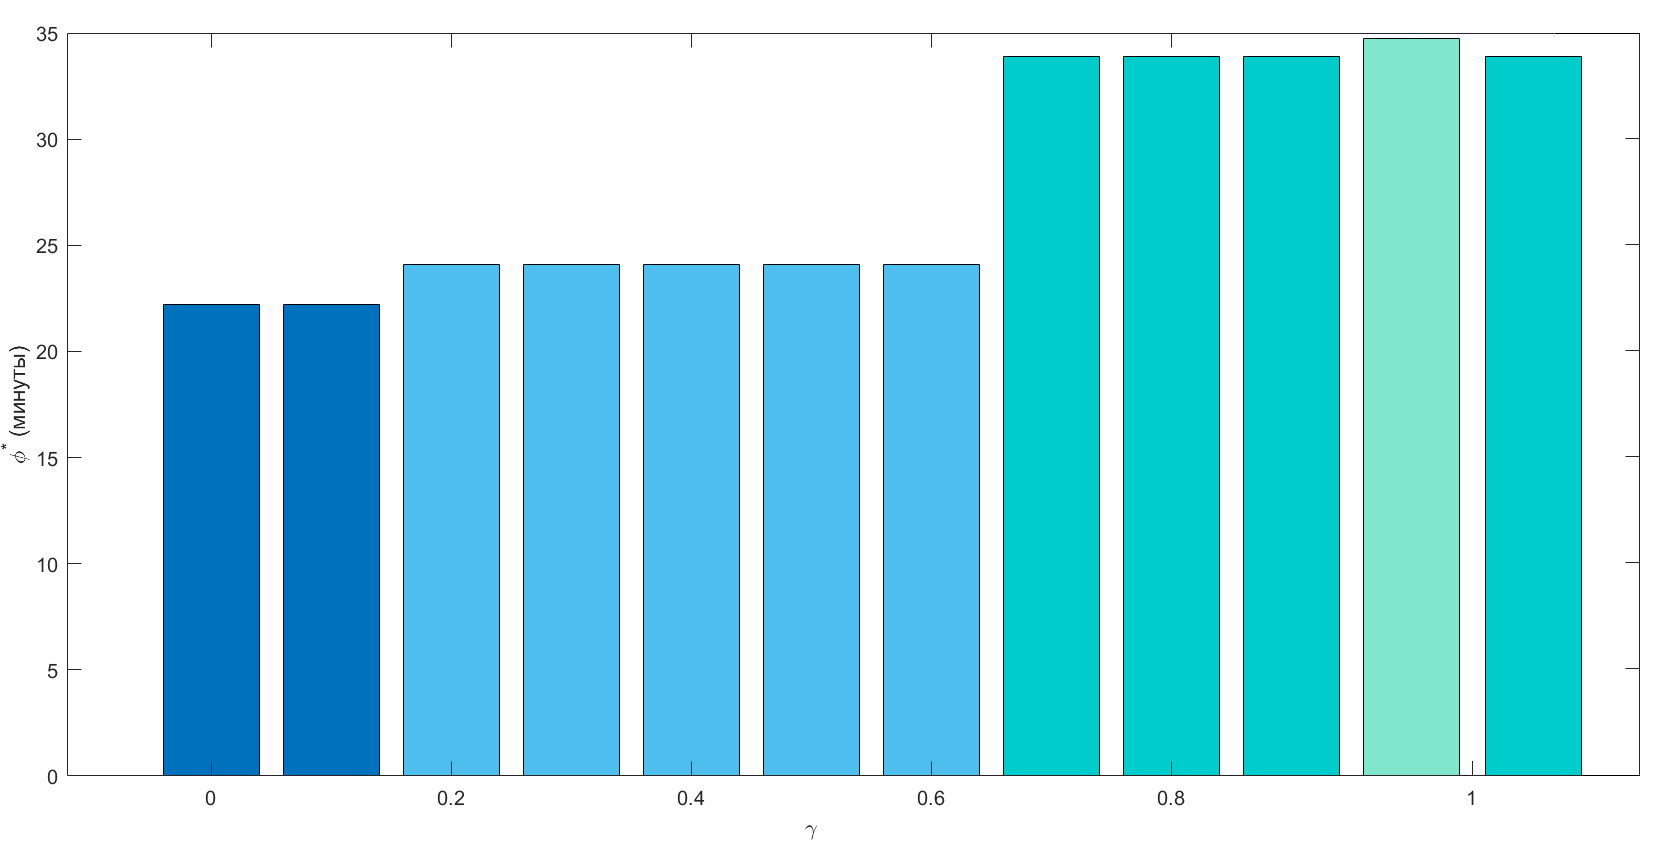
\includegraphics[scale=0.38]{2.png}
Рис. 2.1 Квантили времени выполнения подобранных тестов для $\varepsilon=0.005$
\end{center}



\newpage
Совместное время выполнения предложенных алгоритмов 1.6 и 2.1 составило 255.647838 секунд для всех значений $\varepsilon=0.001,\ldots,0.005$ и всех значений $\gamma=0,\ldots,1$. Время, затраченное на решение задачи для фиксированных значений параметров $\varepsilon$ и $\gamma$, не превышает 2 минут, оно приведено в таблице 2.12.
\begin{table}[h!]
\centering
\begin{flushright}
Таблица 2.12 Время выполнения алгоритма
\end{flushright}
\begin{tabular}{|>{\centering}m{100pt}|>{\centering\arraybackslash}m{350pt}|}
\hline
$\varepsilon$   & Затраченное время (секунды) \\ \hline
0.001           & 102.984447    \\ \hline
0.002           & 97.364834     \\ \hline
0.003           & 113.665582    \\ \hline
0.004           & 91.660544     \\ \hline
0.005           & 105.428571    \\ \hline
\end{tabular}
\label{ch2}
\end{table}
}

\begin{table}[h!]
\centering
\begin{flushright}
Таблица 2 Таблица 1 Наборы заданий для минимальных значений критериальной функции для разных значений допустимых отклонений от суммарной сложности теста
\end{flushright}
\scriptsize{
\begin{tabular}{|c|c|c|c|c|c|c|c|c|c|c|}
\hline
	           		 & Кол-во        & \multicolumn{3}{c|}{$\gamma = 0$}	  & \multicolumn{3}{c|}{$\gamma = 0.5$}	& \multicolumn{3}{c|}{$\gamma = 1$}	\\ \cline{3-11}
					 & реш-й,        & \multirow{4}{30pt}{\centering{$\varphi^\ast$ (минуты)}}	&\multirow{4}*{\centering{$\psi^\ast$}} &   			& \multirow{4}{30pt}{\centering{$\varphi^\ast$ (минуты)}}	&\multirow{4}*{\centering{$\psi^\ast$}} &   			 & \multirow{4}{30pt}{\centering{$\varphi^\ast$ (минуты)}}	&\multirow{4}*{\centering{$\psi^\ast$}} &   			  \\
$\varepsilon$		 & удовл.	&     & 	& Номера заданий,	&     &  	& Номера заданий,	&   & 	& Номера заданий,  \\
					 & дет.		& 	  &		& вошедших в тест   &     &		& вошедших в тест   &   & 	& вошедших в тест  \\
					 & огр.		&	  & 	&  					&	  &   	& 					& 	&  	& 				   \\ \hline
\multirow{2}*{0.001} & \multirow{2}*{7} & \multirow{2}*{23.3651}  & \multirow{2}*{0.5192} & \multirow{2}*{$z^1_6, z^2_1, z^2_2, z^2_9, z^3_5$} & \multirow{2}*{33.5329}		& \multirow{2}*{0.5226} & \multirow{2}*{$z^1_6, z^1_{10}, z^2_5, z^3_6, z^3_7$}  & 34.7905 & 0.3000	 & $z^1_5, z^1_8, z^2_3, z^3_7, z^3_9$	  	\\ \cline{9-11}
  					& & & 	& 		&      &		&						& 33.5329		& 0.3000 		& $z^1_6, z^1_{10}, z^2_5, z^3_6, z^3_7	$	\\ \hline
\multirow{2}*{0.002} & \multirow{2}*{21} & \multirow{2}*{23.3651}	& \multirow{2}*{0.5192} & \multirow{2}*{$z^1_6, z^2_1, z^2_2, z^2_9, z^3_5$} & \multirow{2}*{33.5329} & \multirow{2}*{0.5226}	& \multirow{2}*{$z^1_6, z^1_{10}, z^2_5, z^3_6, z^3_7$}
& 34.7905	& 0.1500	& $z^1_5, z^1_8, z^2_3, z^3_7, z^3_9$		\\ \cline{9-11}
					& & & 	& 		&      &		&						& 33.5329		& 0.1500 		& $z^1_6, z^1_{10}, z^2_5, z^3_6, z^3_7$	\\ \hline
\multirow{2}*{0.003} & \multirow{2}*{30} & \multirow{2}*{22.0362}	& \multirow{2}*{0.4897} & \multirow{2}*{$z^1_7, z^1_{10}, z^2_1, z^2_4, z^3_5$} & \multirow{2}*{23.3651}	& \multirow{2}*{0.3929}	& \multirow{2}*{$z^1_6, z^2_1, z^2_2, z^2_9, z^3_5$}	  & 34.7905		& 0.1000		& $z^1_5, z^1_8, z^2_3, z^3_7, z^3_9$		\\ \cline{9-11}		
					& & & 	& 		&      &		&			& 33.5329		& 0.1000		& $z^1_6, z^1_{10}, z^2_5, z^3_6, z^3_7$	\\ \hline					
\multirow{2}*{0.004} & \multirow{2}*{35}		& \multirow{2}*{22.0362}		& \multirow{2}*{0.4897}				& \multirow{2}*{$z^1_7, z^1_{10}, z^2_1, z^2_4, z^3_5$} & \multirow{2}*{23.3651}		& \multirow{2}*{0.3929}        		& \multirow{2}*{$z^1_6, z^2_1, z^2_2, z^2_9, z^3_5$}     & 34.7905		& 0.0750		& $z^1_5, z^1_8, z^2_3, z^3_7, z^3_9$ 		\\ \cline{9-11}
					& & & 	& 		&      &		&			& 33.5329		& 0.0750		& $z^1_6, z^1_{10}, z^2_5, z^3_6, z^3_7$	\\ \hline			
\multirow{2}*{0.005} & \multirow{2}*{40}		& \multirow{2}*{22.0362}		& \multirow{2}*{0.4897}				& \multirow{2}*{$z^1_7, z^1_{10}, z^2_1, z^2_4, z^3_5$} & \multirow{2}*{23.3651}		& \multirow{2}*{0.3929}        		& \multirow{2}*{$z^1_6, z^2_1, z^2_2, z^2_9, z^3_5$}	  & 34.7905		& 0.0600		& $z^1_5, z^1_8, z^2_3, z^3_7, z^3_9$		\\ \cline{9-11}
					& & & 	& 		&      &		&			& 33.5329		& 0.0600		& $z^1_6, z^1_{10}, z^2_5, z^3_6, z^3_7$	\\ \hline	
\end{tabular}
}\par
\label{ch2}
\end{table}

\newpage
\begin{center}
\section*{ЗАКЛЮЧЕНИЕ}
\addcontentsline{toc}{section}{ЗАКЛЮЧЕНИЕ}
\end{center}

В данной магистерской диссертации предлагается исследование математической модели времени ответа пользователей и решение задачи поиска ограниченного по времени теста для группы студентов с заданной суммарной сложностью в виде решения одноэтапной задачи квантильной оптимизации.

За основу модели времени ответа пользователя была взята модель ван дер Линдена. В силу недостатков использования логнормального распределения в сформулированной задаче, был предложен алгоритм подбора параметров гамма-распределения для времени ответа студента на каждое задание. Преимуществом использования такой модели в данной задаче является возможность получения точного значения квантили, в отличии от модели логнормального распределения вектора случайных параметров.

В результате решения задачи с приведенными в магистерской диссертации значениями параметров распределения, сложностей заданий и теста в целом, для каждого значения отклонения сложности подобранного теста $\varepsilon$ и каждого значения весового коэффициента $\gamma$ был получен оптимальный тест. Результаты численного эксперимента подтверждают валидность предложенной модели. Таким образом, был разработан удобный инструмент, который позволяет автоматически подбирать задания для проведения тестирования с учётом поставленных целей. В ходе работы были опубликованы основные результаты исследования, они представлены в трудах [8,9,10].

\newpage
\begin{center}
\section*{СПИСОК ИСПОЛЬЗОВАННЫХ ИСТОЧНИКОВ}
\addcontentsline{toc}{section}{СПИСОК ИСПОЛЬЗОВАННЫХ ИСТОЧНИКОВ}
\end{center}

1.	Босов А.В., Мхитарян Г.А., Наумов А.В., Сапунова А.П. Использование модели гамма-распределения в задаче формирования ограниченного по времени теста в системе дистанционного обучения // Информатика и её применения. - 2019. - Том 13. - № 4. - С. 11–17

2.	Иноземцев А.О., Кибзун А.И. Оценивание уровней сложности тестов на основе метода максимального правдоподобия // Автоматика и телемеханика. - 2014. - №4.

3.	Кибзун А. И., Панарин С. И. Формирование интегрального рейтинга с помощью статистической обработки результатов тестов // Автоматика и Телемеханика. - 2012ю - № 6. - C. 1.19-139.

4.	Кибзун А.И., Иноземцев А.О. Оценивание уровней сложности тестов на основе метода максимального правдоподобия // Автоматика и телемеханика. - 2014. - № 4. - С. 20–37.

5.	Наумов А. В., Мхитарян Г. А. О задаче вероятностной оптимизации для ограниченного по времени тестирования // Автоматика и телемеханика, 2016. - № 9. - C. 124–135.

6.	Наумов А.В., Джумурат А.С., Иноземцев А.О. Система дистанционного обучения математическим дисциплинам CLASS.NET // Вестник компьютерных и информационных технологий. - 2014. - № 10. - C. 36-40.

7.	Наумов А.В., Мхитарян Г.А., Черыгова Е.Е. Задача формирования теста заданного уровня сложности с минимальным временем выполнения // 17-я Международная конференция «Авиация и космонавтика – 2018». 19–23 ноября 2018 года. Москва. Тезисы. - 2018. - С. 480 - 481.

8.	Наумов А.В., Мхитарян Г.А., Черыгова Е.Е. Стохастическая постановка задачи формирования теста заданного уровня сложности с минимизацией квантили времени выполнения // Вестник компьютерных и информационных технологий. - 2019. - № 2. - С. 37–46.

9.	Наумов А.В., Черыгова Е.Е, Сапунова А.П. Одноэтапная задача квантильной оптимизации для формирования ограниченного по времени теста в СДО с использованием гамма-распределения в качестве вероятностной модели случайного параметра // «Гагаринские чтения – 2019»: Сборник тезисов докладов. - 2019. - С. 715.

10.	Наумов А.В., Черыгова Е.Е., Сапунова А.П. Задача поиска наборов заданий для ограниченного по времени тестирования группы студентов // 18-я Международная конференция «Авиация и космонавтика – 2019». 18-22 ноября 2019 года. Москва. Тезисы. - 2019. - С. 200.

11.	Crocker, L.M., \& Algina, J. Introduction to classical and modern test theory. - 1986.

12.	Gulliksen H. Theory of mental tests. New York: Wiley. - 1950.

13.	Lord, F. M., Novick, M. R. Statistical theories of mental test scores // Addison Wesley. - 1968.

14.	Rasch G. Probabilistic models for some intelligence and attainment tests // Chicago: University of Chicago Press. - 1960.

15.	Rob R. Meijer, Leonardo S. Sotaridona, Detection of Advance Item Knowledge Using Response Times in Computer Adaptive Testing // Law School Admission Council Computerized Testing Report. - 2006.

16.	Roskam, E. E. Models for speed and time-limit tests. In W. J. van der Linden \&amp; R. K. Hambleton (Eds.), Handbook of modern item response theory. -  1997. -  P. 187–208.

17.	Roskam, E. E. Toward a psychometric theory of intelligence. In E. E. Roskam \&amp; R. Suck (Eds.) // Progress in mathematical psychology. - 1987.

18.	Shavelson, R.J., \& Webb, N.M. Generalizability theory: A primer // Measurement methods for the social sciences series. - 1991. - Vol. 1.

19.	Spearman C. Correlation calculated from faulty data // British Journal of Psychology. - 1910. - Vol. 3. - № 2. - P. 271–295.

20.	Thissen, D. Timed testing: An approach using item response theory. In D. J. Weiss (Ed.), New horizons in testing: Latent trait test theory and computerized adaptive testing. - 1983. - P. 179–203.

21.	Thurstone L. L. Ability, motivation, and spee. // Psychometrika. - 1937. - №2. - P.249–254.

22.	Van der Linden W. J. A Hierarchical Framework for Modeling Speed and Accuracy on Test Items // Psychometrika. - 2007. - № 72(3). - P. 287–309.

23.	Van der Linden W. J., Scrams D. J., Schnipke D. L. Using response-time constraints to control for speededness in computerized adaptive testing // Applied Psychological Measurement. - 1999. - № 23. - P. 195–210.

24.	Van der Linden W. J., van Krimpen-Stoop E. M. L. A. Using response times to detect aberrant response patterns in computerized adaptive testing // Psychometrika. - 2003. - № 68. - P. 251–265.

25.	Wang T., Hanson B.A. Development and Calibration of an Item Response Model that Incorporates Response Time // American Educational Research Association. - 2001.

26.	Woodbury M.A. On the standard length of a test // Psychometrika. - 1951. - № 16. - P. 103–106.

27.	Woodbury M.A. The stochastic model of mental test theory and an application. - 1963. - № 28. - P. 391–393.



\newpage
\headsep=12cm
\begin{center} \section*{ПРИЛОЖЕНИЯ} \end{center}
\addcontentsline{toc}{section}{ПРИЛОЖЕНИЯ}
\newpage
\headsep=25pt
\begin{flushright}
Приложение 1
\end{flushright}
\begin{center}
Код программы
\end{center}
\small
\begin{verbatim}
clc;
tic;
I=30; % кол-во заданий
M=3; % кол-во типов
k=5;
N=3;
c=29.46;
E=[0.001 0.002 0.003 0.004 0.005];
krit=0;
krit_f=0;
nabor_o=0;
delta_f=0;
PHI = 0;
user_1 = [3.67486818 3.7349134 3.91696025 3.98131335
    4.00642811 4.1699718 4.28303737 4.3145476  4.34199927
    4.3477965  4.48113232 4.51232291 4.62782186 4.69566873
    4.84054926 4.93260376 5.02189008 5.03291227 5.08443544
    5.15819452 5.22524746 5.38316168 5.39166999 5.47559297
    6.00335788 6.02787477 6.05469 6.07602951 6.09554212
    6.14444415 6.23723904 6.55638912 6.6506526  6.79467691
    6.83630527 6.84530033 6.89123811 6.96288068 6.99995892
    7.02001156 7.16478306 7.17546891 7.20913012 7.41089763
    7.41402334 7.4892427  7.5424666  7.67380759 7.75826456
    7.79098893];
user_2 = [3.72280038 3.73240426 3.92381902 4.00220294
    4.01827787 4.20687381 4.44059374 4.45251726 4.459119
    4.57479634 4.58625472 4.75537707 5.06979788 5.21201389
    5.37981099 5.45170944 5.45259533 5.52832519 5.56189533
    5.87038067 5.90135724 5.97621728 6.03615536 6.25036663
    6.28846734 6.32911807 6.43499058 6.47560566 6.51542247
    6.52239412 6.54330422 6.63444426 6.66560361 6.67519932
    6.76444133 6.80321862 6.8167639  6.94857278 6.95297523
    7.31517343 7.44112472 7.47187685 7.5021167  7.52889623
    7.54348772 7.56673285 7.62638552 7.66944782 7.75773972
    7.78107298];
user_3 = [3.6065242  3.64662143 3.7395852  3.74066167
    4.0329882  4.06054233 4.22557641 4.34267054 4.47382132
    4.48815272 4.61823495 4.72602168 4.73768643 4.7604472
    4.92010962 4.95857915 5.02807928 5.24757324 5.30107296
    5.40717746 5.54259986 5.62430622 5.65030515 5.68014447
    5.79588802 5.83922993 5.91178415 5.99788785 6.1737489
    6.17846059 6.24564593 6.34000956 6.48547783 6.72371129
    6.9337268  7.02046294 7.04072044 7.15834661 7.22269794
    7.23859104 7.26579064 7.52109456 7.58089538 7.70181743
    7.72333636 7.80406417 7.89634657 7.90383042 7.9313355
    7.93346339];

sigma=0.31;

GamPar = gamma_params(user_1,sigma,I);
theta1=GamPar(1,I+1);
ki1=GamPar(1,1:I);

GamPar = gamma_params(user_2,sigma,I);
theta2=GamPar(1,I+1);
ki2=GamPar(1,1:I);

GamPar = gamma_params(user_3,sigma,I);
theta3=GamPar(1,I+1);
ki3=GamPar(1,1:I);

w=[1.3113 3.2545 3.2545 3.2545 4.8738 5.3677 7.0109 7.2167 8.2444
    9.6356 4.132 6.9023 2.1219 3.4366 2.4562 5.3587 6.9023 7.2833
    7.8147 9.3991 2 2.4182 2.6666 3.6536 5.2425 5.5474 6.4528
    7.1938 8.7945 3.6571 1.9694 3.1841 3.1841 5.7378 5.7378 6.3872
    6.9135 7.4123 9.6663 9.7777 1.3131 1.3131 1.3131 4.2146 5.0101
    5.3428 5.7649 6.2283 7.4139 9.6678]';
w = w(1:30,1);
alfa = 0.95;

u=zeros(I,1);
e_I=ones(I, 1);
e_M=ones(M, 1);

e=ones(10,1);
z=zeros(10, 1);
A=[e z z ; z e z ; z z e];
R = zeros(1,11);
R1 = zeros(1,11);

gamma=0;%:0.1:1;
[g1,g2]=size(gamma);
for d=1:g2 цикл по гамма
    for s=1:5 %цикл по епсилон
        U = u_eps(I,c,E,w,s); % функция для получения всех
        % наборов заданий соотвествующих конкретному значению
        % эпсилон
        [r,nm]=size(U);
        nabor = zeros(k,nm); % множество наборов заданий
        % для заданого эпсилон

        for i=1:nm
            o=1;
            for j=1:r
                if U(j,i)>0
                    nabor(o,i)=j;
                    o=o+1;
                end
            end
        end

        nabor = nabor';
        [nm,r]=size(nabor);

        X=0:1:7000;
        f=zeros(1,nm);
        phi_alfa=zeros(1,nm);
        for i=1:nm % цикл по комбинациям наборов внутри эпсилон
            Ind12=independence(ki1*U(:,i),ki2*U(:,i),theta1,theta2);
            Ind23=independence(ki2*U(:,i),ki3*U(:,i),theta2,theta3);
            Ind13=independence(ki1*U(:,i),ki3*U(:,i),theta1,theta3);

            if Ind12==true && Ind23==true && Ind13==true
                fprintf(1,'Gam нз \n');
            else
                fprintf(1,'Gam з \n');
            end

            Ind12 = false;
            Ind23 = false;
            Ind13 = false;


            % поиск квантили распределения суммы
            % гамма-распределённых СВ
            % построили график ФР
            FF = gamcdf(X,sum(ki1*U(:,i)),theta1).
                *gamcdf(X,sum(ki2*U(:,i)),theta2).
                *gamcdf(X,sum(ki3*U(:,i)),theta3);
            F = @(x)gamcdf(x,sum(ki1*U(:,i)),theta1)
                *gamcdf(x,sum(ki2*U(:,i)),theta2)
                *gamcdf(x,sum(ki3*U(:,i)),theta3)-0.95;

            % ищем границы отрезка, в котором находится
            % квантиль заданногоуровня
            x1=find(FF - alfa >= 0 & alfa - FF > -0.5);
            x2=find(alfa - FF >=0 & FF - alfa >= -0.5);

            x1=X(1,x1(1,1));
            x2=X(1,max(x2));

            % на графике ФР - alpha в отрезке [x2,x1] находим корень
            phi_alfa(1,i)=fzero(F,[x2,x1]);

            delta1= abs(c-w'*U(:,i));

            f(1,i) = gamma(1,d)*delta1/E(1,s) +
                (1-gamma(1,d))*phi_alfa(1,i)/2700;

            res = [gamma(1,d) E(1,s) phi_alfa(1,i)
                phi_alfa(1,i)/60 nabor(i,:) delta1 f(1,i)];
            R = [R; res];
            krit(1,i) = f(1,i);
        end
        [r,b] = size(krit);
        [g,h] = min(krit(1,:));
        R1 = [R1; R(1+h,:)];
        R = zeros(1,11);
        krit = [];
    end
end
toc

\end{verbatim}

\newpage
\headsep=25pt
\begin{flushright}
\normalsize{Приложение 2}
\end{flushright}
\begin{center}
\normalsize{Функция U\_all}
\end{center}
\small
\begin{verbatim}
function [U]= U_all(I)
u=zeros(I,1);
U=u;

for i=1:I
    for j=i+1:I
        for k=j+1:I
            for l=k+1:I
                for m=l+1:I
                    u=zeros(I,1);
                    u(i,1)=1;
                    u(j,1)=1;
                    u(k,1)=1;
                    u(l,1)=1;
                    u(m,1)=1;
                    U=[U u];
                end
            end
        end
    end
end

U(:,1)=[];
\end{verbatim}
\newpage

\begin{flushright}
\normalsize{Приложение 3}
\end{flushright}
\begin{center}
\normalsize{Функция u\_eps}
\end{center}
\small
\begin{verbatim}
function [U]= u_eps(I,c,E,w,j)

e = ones(10,1);
z = zeros(10, 1);

A=[e z z ; z e z ; z z e];
U1=U_all(I);
U=zeros(I,1);
[l,m] = size(U1);
a = 0;
b = 0;
for i=1:m
    a = c - w'*U1(:,i);
    b = A'*U1(:,i);
    if abs(a)<=E(1,j) && b(1,1)>=1 && b(2,1)>=1
            && b(3,1)>=1%  && b(4,1)>=1 && b(5,1)>=1
        U=[U U1(:,i)];
    end
end
U(:,1)=[];
\end{verbatim}
\newpage

\begin{flushright}
\normalsize{Приложение 4}
\end{flushright}
\begin{center}
\normalsize{Функция independence}
\end{center}
\small
\begin{verbatim}
function [Ind] = independence(k1,k2,theta1,theta2)

l1=0:100:1500;
l2=1600:4000:5600;
l=[l1 l2];

[k,I]=size(k1);
for i=1:I
    x(1,i)=gamrnd(k1(1,i),theta1);
    y(1,i)=gamrnd(k2(1,i),theta2);
end

c=0;
[k,L]=size(l);

for i=1:L
    if i==L
        a=L;
        b=L*1000;
    else
        a=l(1,i);
        b=l(1,i+1);
    end
    for j=1:L
        if j==L
            a2=L;
            b2=L*1000;
        else
            a2=l(1,j);
            b2=l(1,j+1);
        end
        for m=1:I
            if i==L && j==L
                if (x(1,m)>=a && x(1,m)<=b)
                    && (y(1,m)>=a2 && y(1,m)<=b2)
                    c=c+1;
                end
            elseif i==L && j~=L
                if (x(1,m)>=a && x(1,m)<=b)
                    && (y(1,m)>=a2 && y(1,m)<b2)
                    c=c+1;
                end
            elseif j==L && i~=L
                if (x(1,m)>=a && x(1,m)<b)
                    && (y(1,m)>=a2 && y(1,m)<=b2)
                    c=c+1;
                end
            else
                if (x(1,m)>=a && x(1,m)<b)
                    && (y(1,m)>=a2 && y(1,m)<b2)
                    c=c+1;
                end
            end
        end
        A(i,j)=c;
        c=0;
    end
end

Ax=sum(A');
Ay=sum(A);

Ind=true;
p=0;

for i=1:L
    for j=1:L
        if Ax(1,i)*Ay(1,j)~=0
            p = p + ((A(i,j)- (Ax(1,i)*Ay(1,j)/50))^2)/
            (Ax(1,i)*Ay(1,j));
        end
    end
end
p=p*I;
T=chi2inv(0.95,(L-2)^2);

if p<T
    Ind = true;
else
    Ind = false;
end
\end{verbatim}

\end{document}

